% rubber: depend aesbrief-voorbeeld.tex
\documentclass{article}

\usepackage[dutch]{babel}
\usepackage{url,hyperref,enumitem}
\usepackage{a4wide}
\usepackage{aes,cursus}

\setlength\parindent{0cm}
\setlength\parskip{1ex}

\setdescription{style=nextline}

\newcommand\meta[1]{\placeholder[#1]}
\newcommand\marg[1]{\cmdarg{\meta{#1}}}

\newcommand\bladiebla{\begin{slshape}{Rik}\end{slshape}}

\newcommand\classnaam{notulen}% Hier de naam van de class van de handleiding
\newcommand\classsf{\textsf{\classnaam}}
\newcommand\funktie{notulen}% Hier de functie van de class (brief, notulen, ed)

\title{De \classsf-class} %\\{\large versie \fileversion}}
\author{\aeskwadraat \TeXniCie\\\newcommand{\R}{\naam{Rik}}
\url{hektex@a-eskwadraat.nl}}
%\date{\filedate}

\begin{document}

\maketitle


\section{Introductie}%Korte uitleg van het doel van het Package, voorbeeld van aesbrief

De \classsf-class vormt de standaard \funktie \ van \aeskwadraat.
Dit document legt uit hoe je \funktie \ maakt en hoe de verschillende commando's werken.


\section{De class laden}

Met \cmd{documentclass}\cmdarg[opt]{\meta{opties}}\cmdarg{\classnaam} bovenaan je document laad je de \classsf-class.
De \meta{opties} (gescheiden door komma's) zijn:

\begin{description}
\item[Opties voor \classnaam] De optie die je kan meegeven is ``english''. Hiermee veranderen de hele notulen naar het engels.
\end{description}

Overige opties worden doorgegeven aan de article-class.

\section{Informatie opgeven} % Uitleg over de specifieke informatie die opgegeven moet worden voor de class

Er zijn allerlei dingen die je kunt of moet instellen. Dat gebeurt door middel van allerlei commando's die je vrijwel overal tussen \class{\classnaam}
en \cmd{opening} (zie sectie \ref{sec:handleiding}) kunt plaatsen.

Een van de eerste commando's die handig is in de Notulenclass zijn de commando's voor namen. Deze moeten we echter wel eerst zelf maken! Dit gebeurt als volgt: \\

\cmd{newcommand} \cmdarg{\textbackslash Riknaam} \cmdarg{\cmd{naam}\cmdarg{Rik}} \\

Nu kun je met het commando \cmd{Riknaam} automatisch \bladiebla{} laten uitschrijven. Zeker met langere namen scheelt dit veel tijd aan het eind! Let wel op dat de afkorting niet al bestaat, \LaTeX{} begint dan vanzelf te piepen. \LaTeX{} zal automatisch alle volgende tekst er aan vastplakken tenzij je het als volgt gebruikt: \cmd{Riknaam }\cmdarg{}
In dit voorbeeld is het natuurlijk onzinnig om een langer commando dan de naam zelf te gebruiken, maar \cmd{Al}\cmdarg{} is een stuk korter dan Alexander! \\
Dit is ook wat het commando \cmd{korteapnaam} doet. \cmd{korteapnaam} werkt alleen niet samen met \cmd{aplijstpp}. Om korteapaam te te gebruiken gebruik je: \cmd{korteapnaam}\cmdarg{kortenaam}\cmdarg{langenaam}.

\newpage
\subsection{Verplicht}

Binnen de \classnaam class zijn er geen opties verplicht om aan te zetten!

\subsection{Optioneel}

De volgende commando's kun je gebruiken om optionele informatie op te geven.

\begin{description}
\item[\cmd{titel}\marg{Hoe je de notulen wilt titelen}] Zorgt automatisch voor een mooie titel. Als dit niet wordt ingevuld krijgt het document de standaard titel ``Notulen'' en geeft de compiler een waarschuwing.
\end{description}

\begin{description}
\item[\cmd{datum}\marg{De datum die je wilt dat op het document staat}] Zorgt ervoor dat de datum een mooie plek geeft. Als dit niet wordt ingevuld krijgt het document standaard de datum van vandaag en geeft de compiler een waarschuwing. \verb!\date! werkt niet goed, dus gebruik \verb!\datum!.
\end{description}

\begin{description}
\item[\cmd{aanwezig}\marg{De namen van de aanwezige mensen}] Zorgt voor een mooie aanwezigheidslijst bovenaan het document. Hier kun je ook al je zelfgedefinieerde naamcommando's gebruiken! Als dit niet wordt ingevuld staat er standaard dat allen aanwezig zijn.
\end{description}

\begin{description}
\item[\cmd{afwezig}\marg{De namen van de afwezige mensen}] Zorgt voor een mooie afwezigheidslijst. Deze is standaard leeg. Vergeet ook hier niet de naamcommando's te gebruiken!
\end{description}

\newpage

\section{De handleiding zelf}\label{sec:handleiding}

Binnen de \classnaam class wil je een paar opties eigenlijk altijd gebruiken omdat het er mooi uitziet. Deze staan hierboven geschreven. Verder zijn er nog commandos die de \classnaam echt handig maken.

\begin{description}
\item[\cmd{besluit}\marg{Hetgeen wat besloten is.}] Mocht er met de commissie iets belangrijks besloten zijn, dan kun je dit vaststellen met het besluitcommando. Het wordt dan gelijk klaargezet voor de mooie besluitenlijst aan het eind.
\end{description}

\begin{description}
\item[\cmd{advies}\marg{Hetgeen wat geadviseerd is.}] Vooral nuttig voor adviescommisies. Deze kunnen dit dan in hun notulen zetten zodat bestuursleden hier op kunnen scannen. Het wordt dan gelijk klaargezet voor de mooie adviezenlijst aan het eind.
\end{description}

\begin{description}
\item[\cmd{ahb}\marg{Dat wat naar het bestuur mag.}] Als je als commissie iets hebt dat naar het bestuur moet, dan kan je dit gebruiken. Er komt een mooie lijst aan het bestuur aan het eind.
\end{description}

\begin{description}
\item[\cmd{ap}{\marg{Naam}\marg{Wat de persoon moet doen}}] Dit commando geeft een actiepunt aan de persoon die in het eerste argument wordt opgegeven. Tevens wordt het actiepunt klaargezet voor een mooie lijst onderaan de pagina. Tevens kunnen de namen gescheiden worden door komma's om een actiepunt aan meerdere personen tegelijk toe te wijzen.
\end{description}

\begin{description}
\item[\cmd{besluitenlijst}] Dit commando zet je helemaal onderaan. Hiermee verschijnt er een mooie lijst met alle besluiten die gemaakt zijn.
\end{description}

\begin{description}
\item[\cmd{adviezenlijst}] Dit commando zet je helemaal onderaan. Hiermee verschijnt er een mooie lijst met alle adviezen. 
\end{description}

\begin{description}
\item[\cmd{aanhetbestuur}] Dit commando zet je helemaal onderaan. Hiermee verschijnt er een mooie lijst met alles dat naar het bestuur moet. 
\end{description}

\begin{description}
\item[\cmd{aplijst}] Dit commando zet je ook onderaan. Hiermee verschijnt een lijst met alle actiepunten op volgorde waarvan ze genoemd zijn en wie ze moet uitvoeren. In de praktijk gebruik je echter vaker \cmd{aplijstpp}.
\end{description}

\begin{description}
\item[\cmd{aplijstpp}] Dit commando zet je ook onderaan. Hiermee verschijnt een lijst met alle actiepunten gesorteerd op persoon, en eventueel met wie deze samen gedaan moet worden.
\end{description}

\begin{description}
\item[\cmd{opm}\marg{De opmerking in kwestie}] Dit commando zet een korte opmerking tussendoor netjes neer.
\end{description}



\section{Voorbeeld}

We sluiten af met een voorbeeld.
In figuur \ref{fig:code} zie je een voorbeeld-\LaTeX-bestand. De resulterende \funktie \ zie je in figuur \ref{fig:brief}.

\begin{figure}[ht]
\fbox{%
\begin{minipage}{.9\textwidth}
\verbatiminput{notulenvoorbeeld.tex}
\end{minipage}%
}
\caption{Een voorbeeld van het gebruik van \classsf.}
\label{fig:code}
\end{figure}

\begin{figure}
\fbox{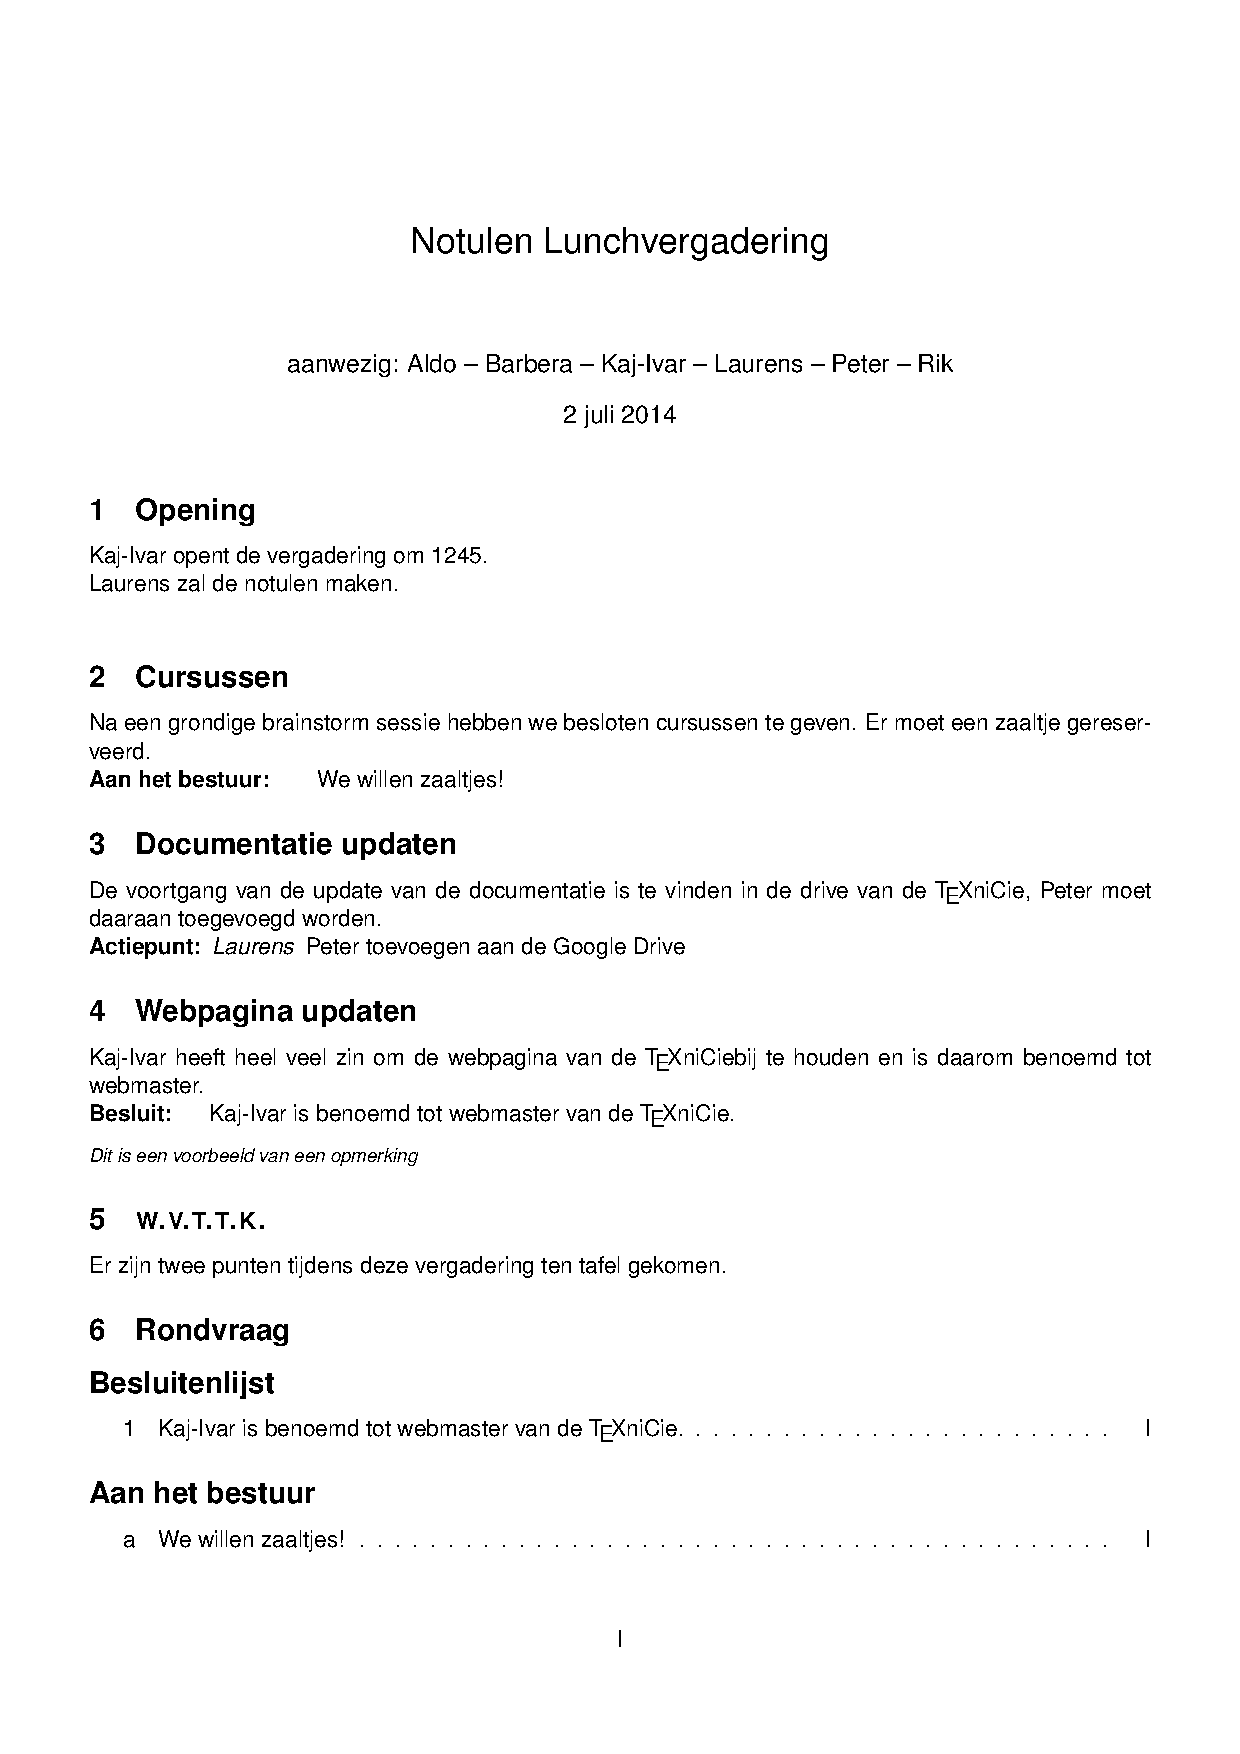
\includegraphics[width=.9\textwidth]{notulenvoorbeeld}}
\caption{De \funktie \ die het resultaat is van de code in figuur \ref{fig:code}.}
\label{fig:brief}
\end{figure}

\end{document}
